\section{Data Sources for Robotic Manipulation}
\label{sec:data}

The quality and diversity of training data are foundational to the generalization ability we seek.
To build such a VLA model with strong generalization across embodiments, tasks, and environments, we curate a large-scale heterogeneous training corpus 
comprising three complementary data modalities: robotic manipulation demonstrations across diverse hardware platforms, egocentric human manipulation videos, and synthetic robot data generated by our human-to-robot pipeline.
A unified curation and pre-processing pipeline processes all sources to ensure high-quality and consistent state, action, video, and language annotations.
Table~\ref{tab:data_overview} summarizes the composition of the full corpus.

% \begin{table}[h]
% \centering
% \caption{\textbf{Overview of the training data corpus.}}
% \vspace{-4pt}
% \label{tab:data_overview}
% \tabcolsep 3pt
% \resizebox{\textwidth}{!}{
% \begin{tabular}{lllll}
% \toprule
% \textbf{Data Type} & \textbf{Embodiment Type} & \textbf{Data Sources} & \textbf{Task Setting} & \textbf{Total Time} \\
% \midrule
% \multirow{3}{*}{Robot} & Single-arm & \makecell{OXE, RoboMIND, DROID,\\ RH20T, InternData-A1} & Tabletop & 3,808 h \\
%                        & Dual-arm  & \makecell{RoboMIND, AgibotWorld-Beta,\\RoboCOIN, RDT, InternData-A1} & Tabletop & 6,744 h \\
%                        & Mobile \& humanoid & \makecell{Galaxea Open-World, RoboCOIN} & Tabletop \& indoor & 868 h \\
% \midrule
% % Human & Human hands & EgoDex, VITRA, EgoVerse & Tabletop \& in-the-wild & 2,686 h \\
% % \midrule
% Human-to-Robot & 15 dual-arm platforms & \makecell{Synthesized from Ant, EgoDex, VITRA, EgoVerse} & Tabletop \& in-the-wild & 25,259 h \\
% \bottomrule
% \end{tabular}}
% \end{table}

\begin{table}[h]
\centering
\caption{\textbf{Overview of the training data corpus.}}
\vspace{-4pt}
\label{tab:data_overview}
\tabcolsep 3pt
\resizebox{\textwidth}{!}{
\begin{tabular}{lllll}
\toprule
\textbf{Data Type} & \textbf{Embodiment Type} & \textbf{Data Sources} & \textbf{Task Setting} & \textbf{Total Time} \\
\midrule
\multirow{3}{*}{Robot}
  & Single-arm         & \multirow{3}{60mm}{\raisebox{-2.9ex}{\parbox{60mm}{\{OXE, RoboMIND, DROID, RH20T, AgibotWorld-Beta, RoboCOIN, RDT, InternData-A1, Galaxea Open-World\}}}}
                                          & Tabletop              & 3,808 h \\[2pt]
  & Dual-arm           &                 & Tabletop              & 6,744 h \\[2pt]
  & Mobile \& humanoid &                 & Tabletop \& indoor    & 868 h   \\
\midrule
Human          & Human hands           & EgoDex, VITRA, EgoVerse      & Tabletop \& in-the-wild & 1,933 h  \\
\midrule
Human-to-Robot & 15 dual-arm platforms & Synthesized from human data. & Tabletop \& in-the-wild & 24,808 h \\
\bottomrule
\end{tabular}}
\end{table}

\subsection{Robotic Datasets}

Robot manipulation demonstrations constitute the core of our pretraining corpus, spanning single-arm and bimanual tabletop manipulation, dexterous manipulation, mobile manipulation, and humanoid loco-manipulation in both simulation and real world.
We incorporate nine open-source datasets, totaling over 11,000 hours of demonstrations.

\textbf{Open X-Embodiment (OXE)}~\citep{padalkar2023openxembodiment} aggregates real-world robotic datasets from diverse research institutions.
We retain three subsets (\emph{Fractal}, \emph{Bridge}, and \emph{BC-Z}) of high-quality single-arm tabletop manipulation data across the Google Robot and WidowX platforms, contributing about 600 hours.

\textbf{AgiBotWorld-Beta}~\citep{bu2025agibotworld} is a large-scale real-world humanoid manipulation dataset collected on the AgiBot G1 bimanual platform. We use datasets collected with grippers, covering about 200 task types and 2,400 hours.

\textbf{RoboMIND}~\citep{wu2024robomind} and \textbf{RoboMIND 2.0}~\citep{wu2025robomind2} provide large-scale real-world datasets covering single-arm, dual-arm, ALOHA~\citep{zhao2023aloha}, and humanoid robots across diverse tabletop manipulation tasks. RoboMIND spans four embodiments including Franka Emika Panda, UR5e, AgileX Cobot Magic V2.0, and Tien Kung humanoid; RoboMIND 2.0 extends coverage to six platforms including Franka, UR5, AgileX, ARX, Tien Kung, and Tian Yi. Together they contribute about 1,400 hours of demonstrations.


\textbf{Galaxea Open-World Dataset}~\citep{galaxea2025openworld} provides $\sim500$ hours of real-world bimanual mobile manipulation demonstrations collected on Galaxea dual-arm robots across diverse household tasks.

\textbf{RoboCOIN}~\citep{wu2025robocoin} is a large-scale multi-embodiment real-world dataset covering a wide range of bimanual and humanoid platforms.
We retain 10 embodiment types including AgiBot G1, Airbot MMK2, Alpha Bot 2, AgileX Cobot Magic, Unitree G1edu, Leju, Realman R1 Lite, Realman RMC-AIDA-L, ALOHA, and Tianqin A2, resulting in about 430 hours of demonstrations.

\textbf{DROID}~\citep{khazatsky2024droid} is an in-the-wild single-arm dataset collected with Franka Panda robots across 86 diverse real-world environments, contributing about 95,000 trajectories totaling 500 hours.

\textbf{RH20T}~\citep{fang2023rh20t} is a large-scale contact-rich real-world dataset spanning 4 embodiments (Flexiv, UR5, Franka, and Kuka) with multi-modal sensing including visual, force-torque, audio, and proprioception. 
It covers 140+ tasks across 42 skill categories, resulting in about 1,100 hours of demonstrations.

\textbf{RDT-1B}~\citep{liu2024rdt1b} provides 29 hours of bimanual manipulation demonstrations collected on the ALOHA platform.

\textbf{InternData-A1}~\citep{tian2025interndataa1} is a large-scale dataset generated in high-fidelity simulation environments, covering various single-arm and dual-arm embodiments across pick-and-place, articulated manipulation, and long-horizon tasks, totaling over 3,600 hours.

%In addition, we collect a proprietary real-world dataset of about 750 hours via teleoperation, comprising bimanual tabletop manipulation demonstrations on dual-arm platforms and loco-manipulation demonstrations on the Unitree G1 humanoid robot. 


\subsection{Egocentric Human Datasets}

Egocentric human hand manipulation data is naturally aligned with the perspective of robot-mounted cameras, serving as an efficient source for expanding manipulation data~\citep{kareer2025egomimic,qiu2025humanoid,egoscale,beingh0,beingh05,easymimic}.
We collect egocentric data from three sources with hand pose annotations.

\textbf{EgoDex}~\citep{egodex}, collected using Apple Vision Pro, contains 338K demonstrations across 194 tabletop manipulation tasks totaling 829 hours of 30\,Hz egocentric video.
It provides SE(3) annotations for 25 joints of both hands per frame, tracked on-device using multiple calibrated cameras and visual--inertial SLAM.
We utilize 732 hours for training.

\textbf{VITRA}~\citep{vitra} performs fully automated 3D hand reconstruction, camera trajectory estimation, and atomic action segmentation on unstructured egocentric videos.
It draws from five video sources: Ego4D~\citep{grauman2022ego4d} (cooking-and-cleaning and general activity subsets), EPIC-KITCHENS~\citep{damen2018epic}, EgoExo4D~\citep{egoexo4d}, and Something-Something~v2~\citep{ssv2}, totalling approximately 1M trajectories.
We utilize the Ego4D and EPIC-KITCHENS subsets, contributing about 247 hours of video.

\textbf{EgoVerse}~\citep{egoverse} is a large-scale collaborative egocentric manipulation dataset spanning 1,362 hours across 1,965 tasks, 240 scenes, and 2,087 demonstrators.
Hand poses (21 keypoints per hand) and 6-DoF head poses are recovered via vision-based methods including visual--inertial SLAM and model-based pose estimation.
We utilize the industry-contributed portion, contributing approximately 954 hours of video.

The three sources collectively amount to approximately \textbf{1,933} hours of video.
All hand poses are converted into a unified representation of MANO~\citep{mano} parameters and 21 keypoints; for sources lacking native MANO annotations, parameters are recovered via optimization-based fitting.

%In addition, we collect a proprietary egocentric dataset \textbf{ANT} of approximately 7 hours, covering bimanual tabletop pick-and-place tasks with frame-level MANO~\citep{mano} parameter annotations generated by a real-time hand reconstruction system.

% The four sources collectively amount to approximately \textbf{1.8M} trajectories and \textbf{1,940} hours of video. All datasets are uniformly converted into MANO parameters 
% $(\mathbf{t}\in\mathbb{R}^3,\;\mathbf{r}\in\mathbb{R}^3,\;\boldsymbol{\theta}\in\mathbb{R}^{45},\;\boldsymbol{\beta}\in\mathbb{R}^{10})$ 
% in the world coordinate system, along with camera intrinsics and extrinsics. 
% Here, $\mathbf{t}$ and $\mathbf{r}$ represent global translation and rotation, 
% $\boldsymbol{\theta}$ denotes the axis-angle poses of 15 joints, and $\boldsymbol{\beta}$ represents the shape coefficients. 
% The 3D coordinates of the 21 hand joints and the 6-DoF pose of the end-effector are derived using forward kinematics. 
% To provide a compact grasp encoding independent of the embodied morphology, 
% we perform PCA on $\boldsymbol{\theta}$ across the entire dataset, 
% compressing it into 10-dimensional \textbf{unified eigengrasp} coefficients 
% $\mathbf{z} = (\boldsymbol{\theta} - \boldsymbol{\mu})\mathbf{V}^\top \in \mathbb{R}^{10}$, 
% where $\boldsymbol{\mu}\in\mathbb{R}^{45}$ is the cross-dataset mean pose, 
% and $\mathbf{V}\in\mathbb{R}^{10\times45}$ consists of the top 10 principal components. 
% The left and right hands are modeled separately.

\subsection{Human-to-Robot Data Synthesis}

\begin{figure}[t]
    \centering
    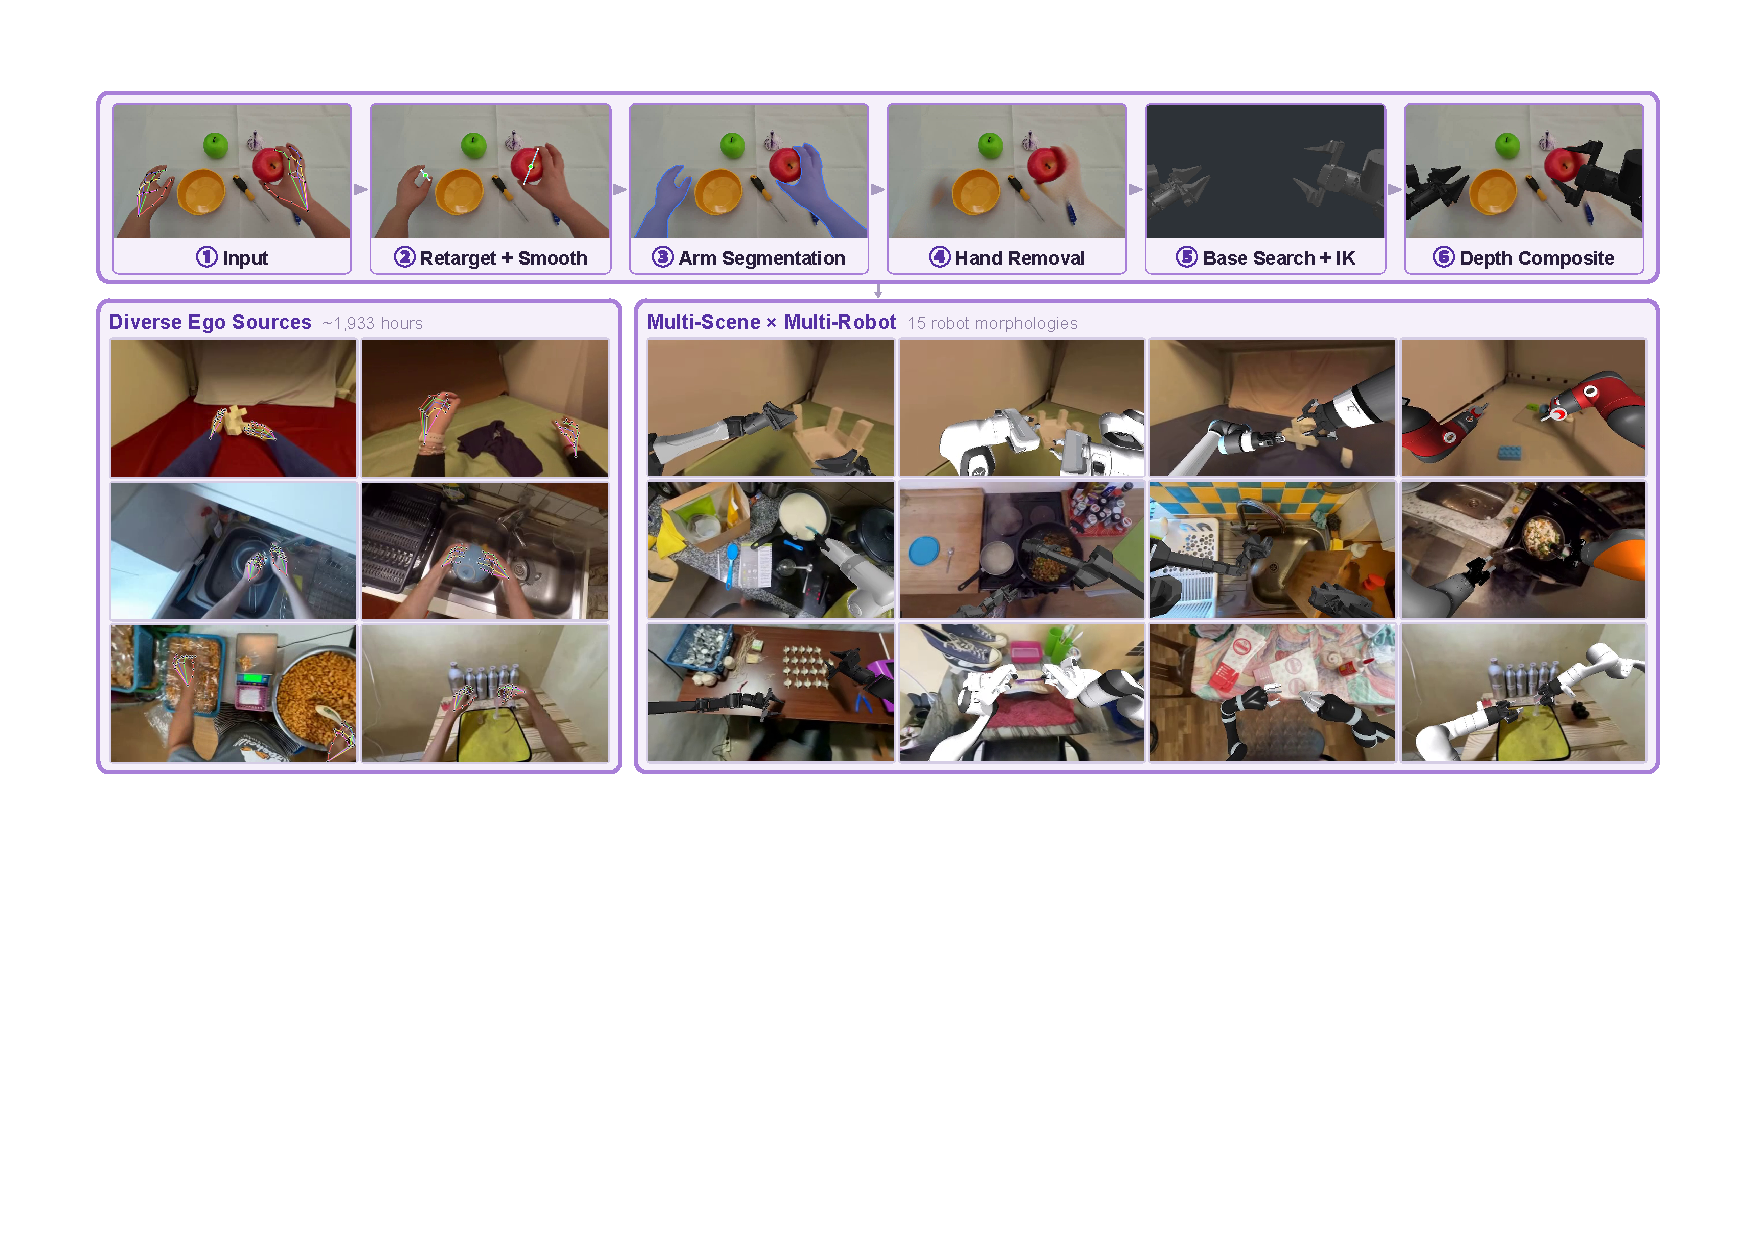
\includegraphics[width=0.98\linewidth]{figures/h2r_pipeline.pdf}
    \vspace{-5pt}
    \caption{\textbf{Human-to-robot data synthesis pipeline.} 
    \textit{(Top)} Given egocentric video, the pipeline performs action retargeting and smoothing, SAM3-based hand segmentation, ProPainter inpainting, base pose search with MuJoCo IK, and depth-guided compositing. 
    \textit{(Bottom)} $\sim$1,933h of egocentric data from 3 sources is rendered across 15 robot morphologies, yielding $\sim$24,808h of synthesized demonstrations.}
    \label{fig:h2r_pipeline}
    \vspace{-1pt}
\end{figure}

% \subsection{Human-to-Robot Data Synthesis}
A significant gap exists between egocentric human data and robot data in both morphology and visual domains. 
To bridge this gap, we map human hand trajectories to the robot action space, and replace human hands in videos with robot models. 
Inspired by prior work~\citep{lepert2025phantom,lepert2025masquerade}, we design an end-to-end synthesis pipeline that explicitly separates the process into action alignment and visual alignment (Figure~\ref{fig:h2r_pipeline}).

\textbf{Action Alignment.} 
This stage focuses on trajectory retargeting and smoothing to bridge the morphology gap between human hands and parallel-jaw grippers.
We define the robot action at frame $t$ as $\mathbf{a}_t = (\mathbf{p}_t,\,\mathbf{R}_t,\,w_t)$, where $\mathbf{p}_t\in\mathbb{R}^3$ is the end-effector position, $\mathbf{R}_t\in SO(3)$ is the gripper orientation, and $w_t\in\mathbb{R}_{\geq 0}$ is the gripper width.
Using the 3D hand keypoints $\mathbf{k}_i$ from MANO, we define a virtual finger $\mathbf{k}_\text{vf}$ as a weighted combination of the index and middle fingertips. 
The end-effector position $\mathbf{p}_t$ is retargeted as the midpoint between the thumb tip and the virtual finger, and the gripper width $w_t$ is their Euclidean distance:
\begin{equation}
  \mathbf{k}_\text{vf} = 0.7\,\mathbf{k}_\text{index} + 0.3\,\mathbf{k}_\text{middle},\quad
  \mathbf{p} = \tfrac{1}{2}\bigl(\mathbf{k}_\text{thumb} + \mathbf{k}_\text{vf}\bigr),\quad
  w = \|\mathbf{k}_\text{thumb} - \mathbf{k}_\text{vf}\|_2.
  \label{eq:eef}
\end{equation}

The gripper orientation is constructed as a right-handed orthonormal frame $\mathbf{R}=[\mathbf{x}\;\mathbf{y}\;\mathbf{z}]$. We first establish the grasp axis $\mathbf{z}$ along the jaw-line direction (the line connecting the thumb tip and the virtual finger). 
Together with the wrist-to-fingertip direction $\mathbf{d}=\mathbf{k}_\text{vf}-\mathbf{k}_\text{wrist}$, these two vectors define the jaw plane; the gripper-normal axis $\mathbf{y}$ is the normal of this plane, and the approach axis $\mathbf{x}$ completes the right-handed frame:
\begin{equation}
    \mathbf{z} = \frac{s \cdot (\mathbf{k}_\text{thumb} - \mathbf{k}_\text{vf})}{w}, \quad
    \mathbf{y} = \frac{\mathbf{z} \times \mathbf{d}}{\|\mathbf{z} \times \mathbf{d}\|}, \quad
    \mathbf{x} = \mathbf{y} \times \mathbf{z}
\end{equation}
where $s=+1$ for the right hand and $s=-1$ for the left hand. This sign flip ensures that $\mathbf{z}$ points in a consistent direction regardless of handedness, so that both hands map to the same gripper frame. The three axes correspond to: $\mathbf{x}$ -- approach direction, $\mathbf{y}$ -- gripper normal (perpendicular to the jaw plane), $\mathbf{z}$ -- grasp axis (along the jaw line).

Per-frame hand detection introduces high-frequency noise. 
We apply Savitzky--Golay~\citep{savitzky1964smoothing} filtering to positions and widths, and Gaussian-weighted SLERP to orientations, producing smooth trajectories while preserving motion structure.

\textbf{Visual Alignment.} 
This stage replaces the human appearance with a robot model through a sequence of masking, inpainting, and rendering steps to bridge the visual domain gap. 
First, SAM3~\citep{carion2025sam3segmentconcepts} generates a binary mask $M_t\in\{0,1\}^{H\times W}$ for the human arm using text prompts. 
Next, ProPainter~\citep{propainter} inpaints the masked regions guided by optical flow, creating a clean background sequence $\{\hat{I}_t\}$ without human hands. 

A fundamental challenge in converting ego videos to robot data is determining the robot base placement. Unlike robot-to-robot transfer where a source base position is available, egocentric hand trajectories are embodiment-free: there is no physical robot base to reference. We formulate this as an optimization over base placements: given $N$ target end-effector poses $\{\mathbf{T}_i^\text{ee}\}_{i=1}^{N}$ and a robot with maximum reach $r_\text{max}$, we seek:
\begin{equation}
    \mathbf{T}_\text{base}^* = \arg\max_{\mathbf{T}_\text{base}} \frac{1}{|\mathcal{K}|} \sum_{k \in \mathcal{K}} \mathbb{1}\left[\text{IK}(\mathbf{T}_\text{base}^{-1} \mathbf{T}_k^\text{ee}) \text{ is feasible}\right]
\end{equation}
where $\mathcal{K} \subset \{1, \dots, N\}$ is a set of representative keyframes covering the spatial extremes of the trajectory. Candidate base placements are generated via grid search around the trajectory centroid, constrained by the per-morphology kinematic reach $r_\text{max}$. 
This search is performed independently for each of the 15 robot morphologies, as different arm lengths and joint configurations require different base placements for the same trajectory.

Given the optimized base pose, we run inverse kinematics in a MuJoCo~\citep{mujoco,Zakka_Mink_Python_inverse_2026} virtual environment to track the smoothed action trajectory, rendering the robot image $I_t^\text{robot}$ and its depth map $D_t^\text{robot}$. 
Depth Anything v3~\citep{da3} estimates a metric depth map $D_t$ for the scene. 
We compute an occlusion mask $M_t^\text{occ} = \mathbb{1}[D_t^\text{robot} \leq D_t]$ to naturally composite the robot onto the clean background:
\begin{equation}
  I_t^\text{syn} = M_t^\text{occ} \odot I_t^\text{robot}
                 + \bigl(1 - M_t^\text{occ}\bigr) \odot \hat{I}_t.
  \label{eq:composite}
\end{equation}

Each human demonstration is rendered into 15 bimanual robot configurations (each composed of two identical arms from: Panda, UR5e, ARX-L5, xArm7, Sawyer, Kinova~Gen3, IIWA, Jaco, FR3, UR10e, ViperX, WidowX, Piper, YAM, AgileX ALOHA), yielding approximately \textbf{24,808} hours of synthesized demonstrations in total.

\textbf{Action Speed Alignment.}
Egocentric hand manipulation exhibits significantly higher action speeds than robot teleoperation data. 
To align the action speed distributions, we apply per-source frame subsampling during training to match the robot data speed. 
Specifically, EgoDex is downsampled to 60\% of its original frame rate ($\sim$1.7$\times$ slower), EgoVerse to 45\% ($\sim$2.2$\times$ slower), and ViTRA to 25\% ($\sim$4$\times$ slower).

\begin{figure}[t]
    \centering
    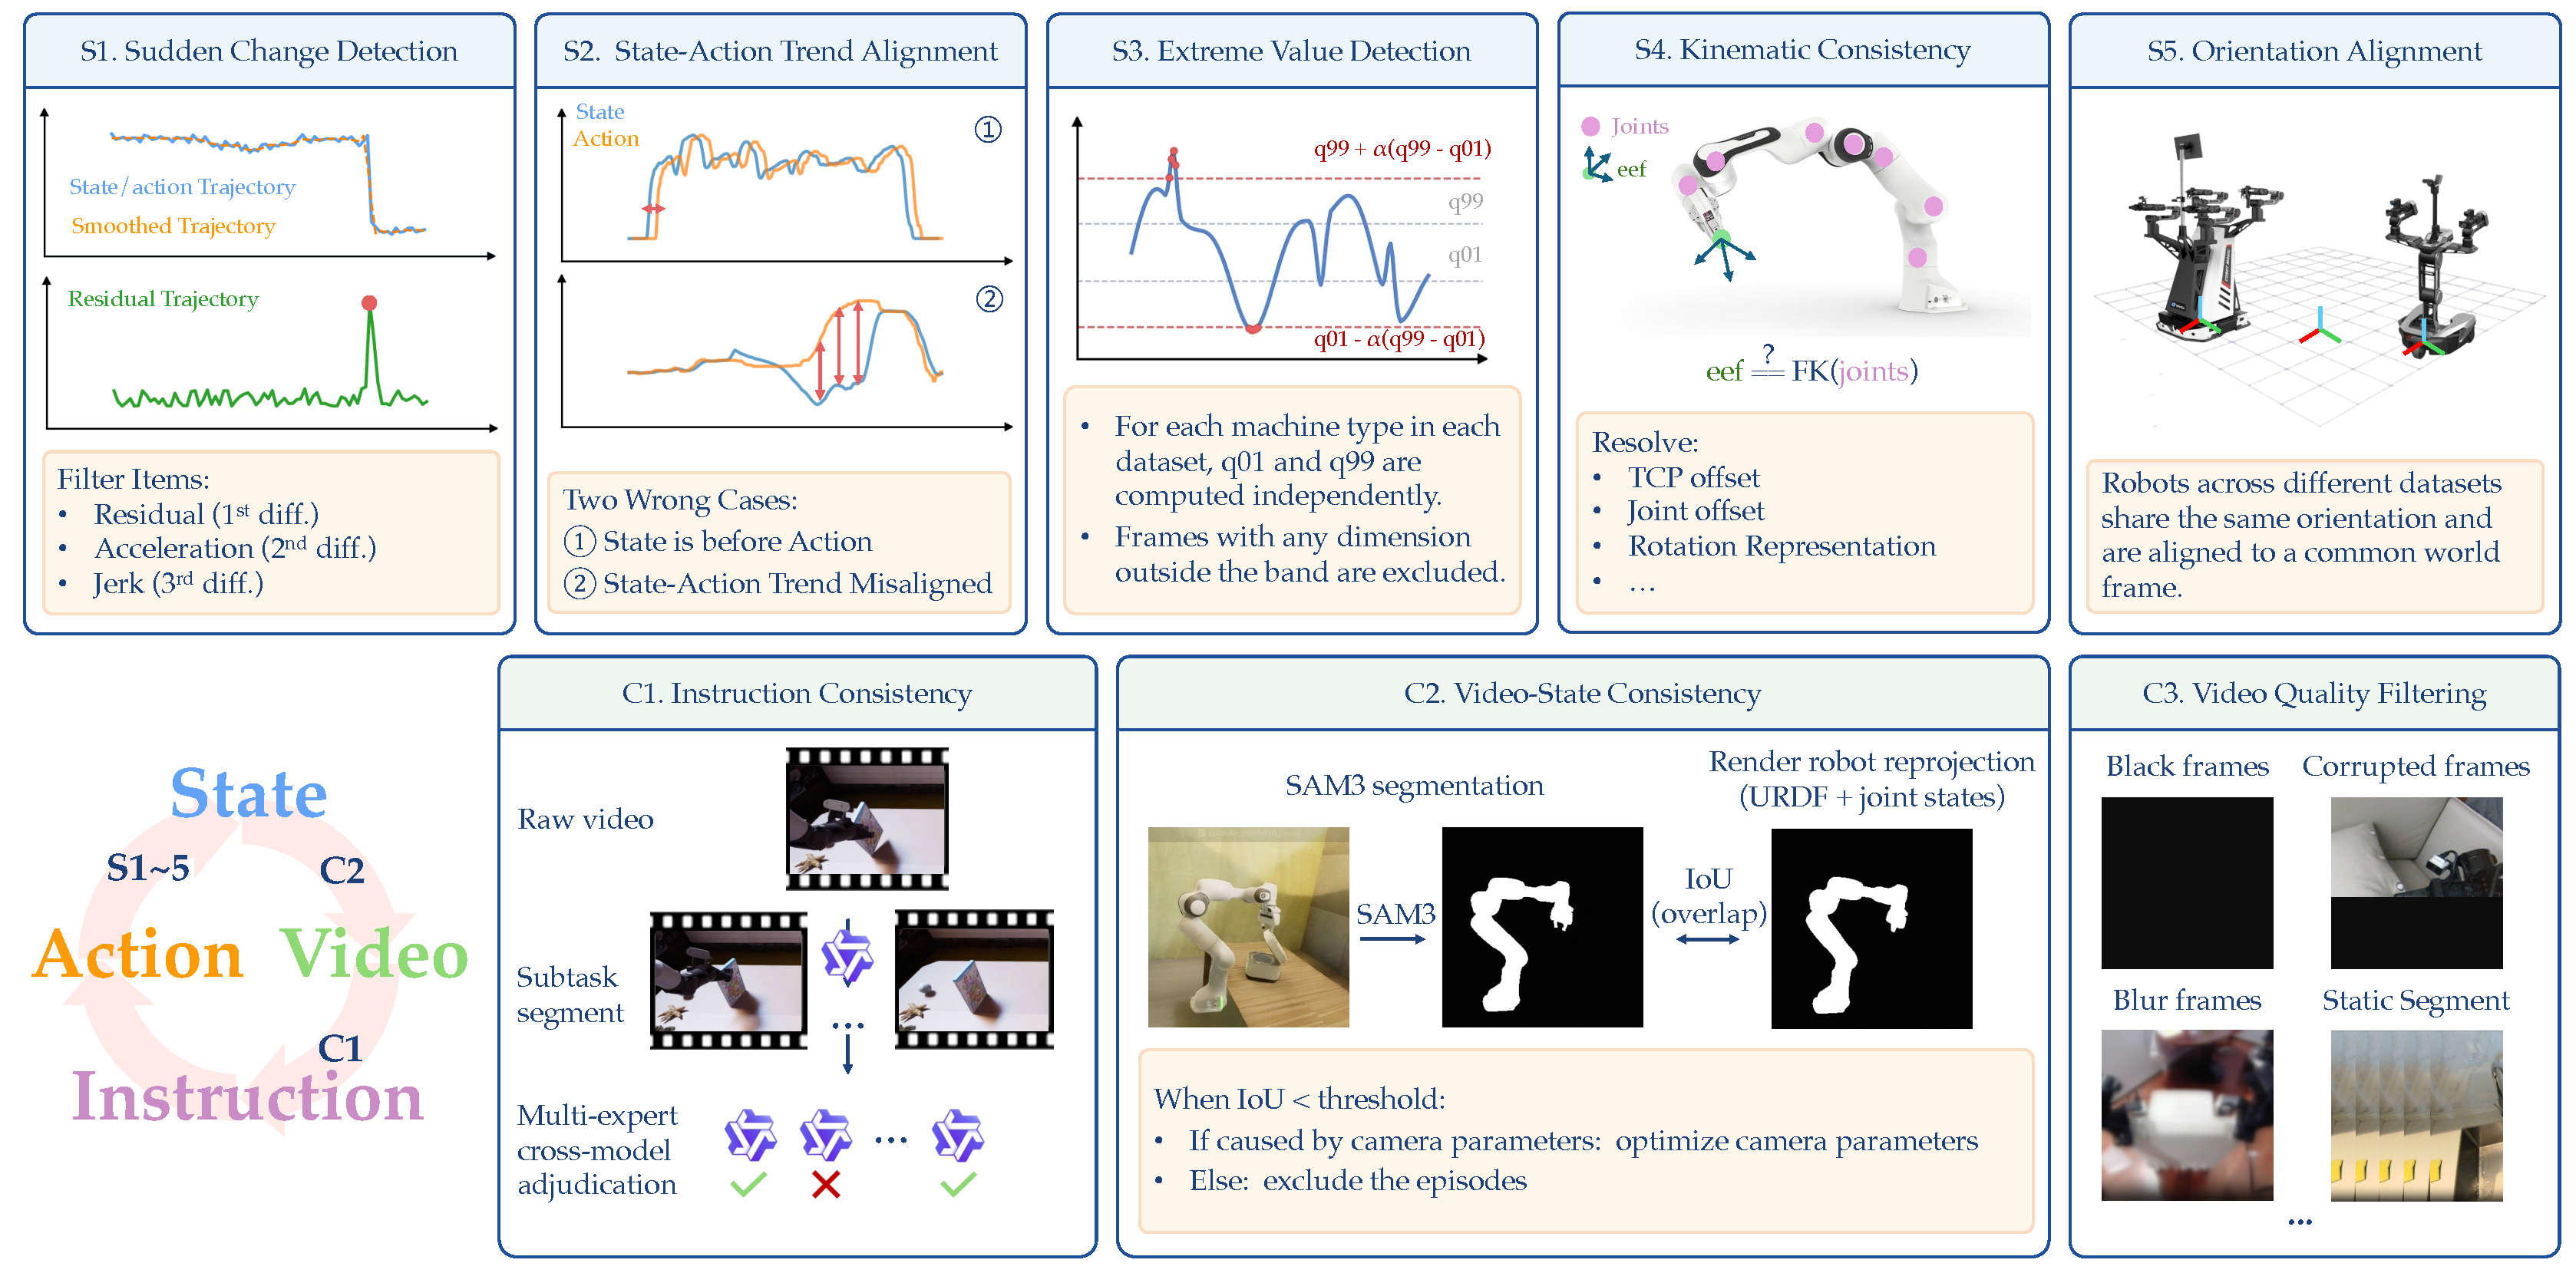
\includegraphics[width=0.98\linewidth]{figures/data_preprocess.pdf}
    \vspace{-3pt}
    \caption{\textbf{Multi-stage data curation pipeline.} Five-stage state-action signal filtering (sudden change, trend alignment, extreme value removal, FK consistency, and base-frame alignment) followed by three cross-modal quality checks (instruction consistency, video-state consistency, and video quality filtering).}
    \label{fig:data preprocess}
    % \vspace{-3pt}
\end{figure}

\subsection{Data Curation and Pre-Processing}
%\subsubsection{State and Action Quality Filtering} 
\label{sec:state_action_filtering}  
Aggregating manipulation data across diverse embodiments, simulators, and collection pipelines introduces heterogeneous noise in recorded state and action signals, including discrete outliers from physical collisions, temporal misalignment between state and action streams due to unsynchronized clocks or packet loss, extreme values that destabilize optimization, and inconsistent end-effector conventions across datasets sharing the same robot embodiment. We address these through a five-stage filtering pipeline applied to all datasets prior to training. 

\paragraph{Stage 1: Sudden Change Detection.}

For each signal dimension, we extract a smooth trend via cascaded median filtering and Savitzky--Golay smoothing~\citep{savitzky1964smoothing}, then compute three complementary deviation signals: the absolute residual between the raw and smoothed trajectory, the second-order finite difference (acceleration), and the third-order finite difference (jerk). A frame is flagged when the residual exceeds a scaled threshold \emph{and} either acceleration or jerk also exceeds its threshold, reducing false positives from slow drift while preserving sensitivity to abrupt transients. Thresholds are set per dataset according to embodiment type, rotation representation, data source (real vs.~simulation), and base mobility. Exclusion strategies range from frame-level removal to full episode discard. For instance, in InternData-A1~\citep{tian2025interndataa1} where sudden changes arise exclusively from physical collisions (\eg, a gripper contacting a rigid object), the corrupted episode is discarded entirely.

  % The first stage identifies discrete outliers and transient discontinuities in both joint and end-effector state-action trajectories. For each dimension of each signal, we first extract a smooth trend via cascaded median filtering and Savitzky--Golay smoothing, then compute three complementary deviation signals: the absolute residual between the raw and smoothed trajectory, the second-order finite difference (acceleration), and the third-order finite difference (jerk). A frame is flagged as anomalous when the residual exceeds a scaled threshold \emph{and} either the acceleration or jerk also exceeds its respective threshold, reducing false positives from slow drift while preserving sensitivity to abrupt transients. The per-key thresholds are set separately for each dataset according to embodiment type, end-effector rotation representation (Euler angles, quaternion, or rotation vector), data source (real vs. simulation), and base mobility (fixed vs. mobile), and are calibrated through manual inspection of flagged episodes.   After identifying anomalous frames, we apply dataset-specific exclusion strategies that range from frame-level removal to full episode discard, depending on the nature of the anomaly. For instance, in simulation datasets such as InternData-A1~\citep{tian2025interndataa1}, trajectories are generated via optimization and sudden changes arise exclusively from physical collisions (e.g. a gripper contacting a rigid object), so the corrupted episode is discarded entirely.

\paragraph{Stage 2: State-Action Trend Alignment.}
In a correctly recorded episode, action commands should temporally lead or coincide with resulting state changes, which is a causal invariant violated when timestamps are unsynchronized or there is packet loss. 
For each shared joint dimension, we smooth both the state and action trajectories, then estimate the optimal temporal lag via cross-correlation, then compute a \emph{directional agreement} (DA) metric on lag-aligned first-order differences. 
Dimensions with DA below a dataset-specific threshold (typically $0.6$-$0.7$) are flagged and their episodes excluded. For datasets using delta actions, we first integrate the action sequence to recover absolute values before comparison. This stage revealed severe quality issues in certain subsets: 81\% of episodes in the RoboMIND UR-type data failed this check and were excluded.

  % The second stage verifies the trend consistency between state and action trajectories over time. In a correctly recorded episode, action commands should temporally lead or coincide with the resulting state changes---a causal invariant that is violated when timestamps are unsynchronized or when bandwidth limitations cause packet loss. For each shared joint key, we smooth both the state and action trajectories, then estimate the optimal temporal lag by maximizing cross-correlation over a search window. We then compute a \emph{directional agreement} (DA) metric on the lag-aligned first-order differences: at each frame where either signal changes by more than a minimum threshold~$\epsilon$, we check whether the signs of the state and action derivatives agree. Dimensions with DA below a dataset-specific threshold (typically $0.6$--$0.7$) are flagged, and episodes containing flagged dimensions are excluded. For datasets that use delta-parameterized actions, we first integrate the action sequence to recover absolute values before comparison. This stage revealed significant quality issues in certain subsets: for example, 81\% of episodes in the RoboMind UR-type data exhibited state--action misalignment and were excluded from training.

\paragraph{Stage 3: Extreme Value Filtering.}
Frames with state or action values outside the expected range are removed to prevent distortion of the quantile-based normalization ($[q_{01}, q_{99}] \to [-1, 1]$) used during training. Per-dimension $q_1$ and $q_{99}$ percentiles are computed per embodiment type, and frames outside the band $[q_1 - \alpha(q_{99}-q_1),\ q_{99}+\alpha(q_{99}-q_1)]$ are excluded. Gripper dimensions are exempt due to their bimodal distributions.

  % The third stage removes frames whose state or action values fall far outside the expected range, which would otherwise distort the quantile-based normalization ($[q_{01}, q_{99}] \to [-1, 1]$) used during training or cause gradient instability. For each embodiment type, we aggregate all episodes across dataset splits sharing the same robot model and compute per-dimension $q_1$ and $q_{99}$ percentiles over both state and action channels. Frames containing any dimension outside the band $[q_1 - \alpha \cdot (q_{99} - q_1),\; q_{99} + \alpha \cdot (q_{99} - q_1)]$ are excluded, where $\alpha$ controls the tolerance margin. Gripper-related dimensions are excluded from this filter, as their bimodal distributions do not conform to percentile-based assumptions.

\paragraph{Stage 4: Joint-End-Effector Forward Kinematics Consistency.}
We compute forward kinematics (FK) via Pinocchio~\citep{carpentier2019pinocchio} from each robot's URDF and compare against logged end-effector poses. The discrepancies can arise from differing joint-angle sign conventions, differing end-effector frame definitions, incorrect rotation representations, incorrect base-frame assumptions, and erroneous end-effector logging. Rather than aggressively filtering, this stage primarily performs \emph{data correction}: constant positional offsets are resolved by adjusting the tool-center-point (TCP) definition, and shoulder-relative bimanual poses are transformed into the world frame. This process revealed that the same robot model can carry different joint-angle conventions across datasets, further motivating the unified state-action representation of Sec.~\ref{sec:unified_state_action}.

  % The fourth stage validates the consistency between recorded joint states and end-effector poses by computing forward kinematics (FK) from the corresponding URDF model and comparing the result against the logged end-effector position and orientation. We first catalog all robot models appearing across datasets and locate their URDF files. For each episode, we construct the joint configuration vector---handling per-dataset joint orderings, sign conventions, and fixed joints---and compute FK via Pinocchio~\citep{carpentier2019pinocchio}. Discrepancies between FK-derived and recorded end-effector poses can arise from five sources: differing joint-angle sign conventions, differing end-effector frame definitions, incorrect rotation representations, incorrect base-frame assumptions, or erroneous end-effector logging. Rather than aggressively filtering, this stage primarily performs \emph{data correction}: if the FK-derived and recorded end-effector poses exhibit a constant positional offset, we adjust the tool-center-point (TCP) definition without discarding the episode; if bimanual end-effector poses are recorded relative to each shoulder rather than the world frame, we transform them into the world frame. During this process, we found that even the same robot model can have different joint-angle conventions across datasets---and in some cases, different tasks within the same dataset exhibit different rotational offsets for the same robot. These findings further motivate the adoption of a unified state-action representation (\cref{sec:unified_state_action}).

\paragraph{Stage 5: Base Frame and End-Effector Orientation Alignment.}
We apply per-dataset rotation corrections to align world-frame orientation conventions, ensuring the positive $x$-axis consistently corresponds to the robot's forward-facing direction and that the unified state-action representation is geometrically consistent across embodiments.

    % The fifth stage aligns the world-frame orientation conventions across different robot setups to ensure that the positive $x$-axis consistently corresponds to the robot's forward-facing direction. Different data collection environments record poses in varying world frames depending on sensor placement and calibration conventions. We apply per-dataset rotation corrections to transform all end-effector poses into a canonical frame where the $x$-axis aligns with the robot's forward direction, ensuring that the unified state-action representation is geometrically consistent across embodiments. 

Beyond this five-stage state and action signal quality filtering, we apply three additional checks to ensure cross-modal consistency across video, language, and proprioceptive observations.

%\subsubsection{}

\paragraph{Check 1: Instruction Consistency.} 
We verify semantic consistency between each demonstration and its language annotation via a three-stage VLM-based pipeline. First, long episodes are decomposed into subtask-level segments~\citep{lei2026towards} so that each clip corresponds to a temporally localized action unit, keeping the visual evidence focused and tractable for automated assessment (Temporal Normalization for Evaluation Units). Second, each segment is evaluated through structured reasoning-guided prompting: rather than requesting an immediate binary label, the VLM is directed to attend to manipulated objects, action semantics, temporal ordering, and agent-environment interaction, producing an intermediate analytical judgment before issuing a final consistency decision. This structured prompting reduces superficial or heuristic responses and improves label interpretability (Structured Reasoning-Guided Annotation). Third, clips flagged as non-aligned or ambiguous by the initial model are adjudicated by multiple VLMs as independent evaluators, with the final label determined by cross-model voting, reducing single-model bias and improving label robustness (Multi-Expert Cross-Model Adjudication). Inconsistent samples are excluded from training.


% The Instruction consistency labeling pipeline is organized around three complementary principles. Temporal Normalization for Evaluation Units ensures that each sample presented to the annotator model lies within a reasonable duration range, so that the visual evidence remains focused and cognitively tractable for VLM's  automated assessment. Overly long videos are therefore decomposed into subtask-level segments, allowing each clip to correspond to a temporally localized action unit rather than an entire extended episode. Structured Reasoning-Guided Annotation then frames consistency checking as a controlled decision process rather than a direct binary prediction. Instead of asking the vision–language model for an immediate label, the pipeline guides it to attend to key aspects of alignment such as manipulated objects, action semantics, temporal ordering, and agent–environment interaction and to produce an intermediate analytical judgment before issuing a final consistency decision. This structured prompting strategy improves interpretability and helps reduce superficial or heuristic responses. Finally, Multi-Expert Cross-Model Adjudication is used to improve reliability on difficult or potentially misaligned samples. When a clip is identified as non-aligned or suspicious by an initial model, multiple vision–language models are further employed as independent evaluators, and the final label is determined through cross-model voting or agreement-based adjudication. This expert-style review mechanism reduces the risk of single-model bias and makes the resulting labels more robust. Taken together, these three components transform consistency checking from a simple one-pass classification task into a staged and quality-aware annotation framework, enabling more reliable identification of semantically consistent data for dataset cleaning, quality control, and downstream training selection.

\paragraph{Check 2: Video-State Consistency.} 
We perform rigorous data cleaning to remove low-quality or misaligned samples.
To verify video-state consistency, we render the robot projection into the image plane using the URDF and recorded joint states, segment the actual robot mask with a fine-tuned SAM3~\citep{carion2025sam3segmentconcepts} model, and measure their overlap. Samples with low overlap are filtered out.

% We perform rigorous data cleaning to remove low-quality or misaligned samples. Since the video stream and robot states are captured by different sensors, temporal or geometric misalignment may occur. To verify cross-modal consistency, we render the robot projection in the image plane using the robot URDF and recorded state values, and segment the robot mask in the observed image with a fine-tuned SAM3~\citep{carion2025sam3segmentconcepts} model. We then measure the overlap between the rendered projection and the segmented mask to determine whether the visual observation and state data are properly aligned. Samples with low overlap are filtered out. 

%\subsubsection{Video Quality Filtering} 
\paragraph{Check 3: Video Quality Filtering}
We apply video-level data cleaning to remove frames that may degrade policy learning. We remove visually invalid frames including black, corrupted, blurred, and prolonged static segments, using image processing checks applied jointly with state and action signals to detect redundant static periods typically at episode boundaries. Task-critical key frames such as gripper closure events are explicitly preserved to avoid discarding visually subtle but semantically important transitions.

% We apply video-level data cleaning to remove frames that may degrade policy learning, including black frames, corrupted frames, blurred frames, and prolonged static segments. Using digital image processing, we filter visually invalid or low-quality frames, while jointly checking video observations with the corresponding state/action signals to identify redundant static periods, which typically occur at the beginning or end of demonstrations. Removing such segments reduces the model’s tendency to learn inactive or hesitant behavior. 

% During static-frame filtering, we explicitly preserve task-critical key frames, such as gripper closure and other decisive state transitions, to avoid discarding visually subtle but semantically important events. This procedure improves data quality while maintaining essential task information.

   


% Data cleaning pipeline ...

% Camera and end-effector processing ...

% Instruction relabeling ...

\subsection{Vision-Language Co-training Datasets}
\label{sec:vlm_data}

Prior works have demonstrated that co-training VLAs with vision-language (VL) data mixtures can significantly improve their generalization ability~\citep{pi05, driess2025knowledge, fang2026molmoact2}. By incorporating VL data during VLA training, the model retains the rich visual and semantic knowledge acquired from web-scale multimodal pretraining and transfers this knowledge to action generation through the action expert. For example, this enables the model to follow novel language instructions, operate in unfamiliar scene backgrounds, or manipulate previously unseen objects.

To this end, we curate a comprehensive VL dataset from multiple sources, including proprietary data, open-source datasets (e.g., RoboPoint~\citep{yuan2024robopoint}, RefSpatial~\citep{zhou2025roborefer}, PixMo~\citep{deitke2025pixmo}, and CapsFusion~\citep{yu2024capsfusion}), and carefully
synthesized embodied-centric data. The resulting VL mixture comprises approximately 28M data points, spanning the following categories:

(1) \textbf{General Visual Understanding}, including visual question answering, multi-image reasoning, and image captioning at varying granularities (from single-sentence summaries to paragraph-level detailed descriptions), which preserves the model's broad visual perception and commonsense reasoning capabilities;

(2) \textbf{Spatial Perception and Reasoning}, covering 2D/3D visual grounding, point localization, counting, spatial relationship reasoning (depth comparison, distance estimation, camera viewpoint inference), and manipulation feasibility reasoning, which are directly transferable to robotic spatial understanding;

(3) \textbf{OCR and Document Understanding}, which helps maintain the VLM's ability to recognize text, numbers, and symbols, a capability that is also required in robotic tasks involving labeled objects (e.g., identifying a block marked with a specific number);

(4) \textbf{Multimodal Specialized Knowledge}, covering domain-specific visual reasoning tasks such as STEM problem solving, chart interpretation, and visual puzzle reasoning, which helps prevent catastrophic forgetting of the VLM's general multimodal reasoning capabilities during VLA fine-tuning;

(5) \textbf{Instruction Following, Multilingual, and Pure Text data}, which strengthens the model's ability to follow diverse natural language instructions, a capability that is critical for generalizing to novel robot tasks, while also enabling multilingual robot control and preserving text generation quality;

(6) \textbf{Embodied-Centric VL Data}, which we specifically curate to bridge the gap between web-scale VL knowledge and robotic manipulation. This subset includes:   (a) embodied chain-of-thought (ECoT) reasoning data derived from robot manipulation trajectories, where the model performs structured reasoning in three stages: first describing the current scene state from multi-view observations (including gripper status, object positions, and spatial layout), then assessing task progress by comparing the current state against the overall goal, and finally predicting the next atomic manipulation action; (b) egocentric video understanding data, where the model describes fine-grained hand/arm movements, hand-object interactions, and object state changes from short clips of first-person human manipulation videos; and (c) 2D trajectory prediction data, where the model predicts future movement trajectories of human hands or robot end-effectors as sequences of normalized 2D coordinates, conditioned on visual observations and task instructions.

Among these, categories (1)–(5) serve a dual purpose: they prevent catastrophic forgetting of the pretrained VLM's general capabilities, while certain subsets, such as spatial reasoning, visual grounding, and OCR, directly benefit robotic manipulation by strengthening the model's spatial understanding, object recognition, and scene generalization. Category (6) is specifically curated to bridge VL understanding and action generation: ECoT data teaches the model to perceive embodiment-specific scene states, track task progress, and reason about next actions in language. This encourages the VLM backbone to build richer embodied representations that are more directly useful for downstream continuous action generation~\citep{zawalski2024robotic, Chen2025TrainingSF}; egocentric video data exposes the model to fine-grained human manipulation patterns and object state transitions from a first-person perspective, grounding its understanding of how physical interactions unfold, including how objects deform, slide, or topple under contact and how hand-object configurations evolve during grasping, placing, and tool use. This knowledge transfers to robotic manipulation despite the embodiment gap. In addition, 2D trajectory prediction data directly connects visual observations to spatial motion reasoning in image coordinates, and together these data sources establish a shared representational foundation that facilitates knowledge transfer to low-level action prediction through the action expert.


% (i) \textbf{Visual grounding} --- 2D and 3D object localization data, which maintains the model's ability to identify and spatially ground objects in a scene.

% (ii) \textbf{OCR} --- text recognition and document understanding data, which preserves fine-grained visual perception and text-reading ability.

% (iii) \textbf{General VQA and captioning} --- visual question answering, image captioning, counting, and spatial reasoning data, which help retain broad scene understanding.

% (iv) \textbf{Instruction following} --- pure-text and image-conditioned instruction-following data in multiple languages, which keeps the model robust to different task phrasings, instruction formats, and multi-linguistic styles.

% (v) \textbf{Embodied reasoning} --- reasoning data specialized for robotic manipulation. Given robot observation images and a task instruction, the model is trained to produce a structured reasoning chain that describes the current scene, assesses task progress, and predicts the next action to take.

We describe the synthesis procedure for each type of embodied-centric VL data below.


\begin{table}[tb]
\centering
\caption{\textbf{Taxonomy of atomic action types.}}
\vspace{-5pt}
\label{tab:atom_actions}
\small
\begin{tabular}{llL{9.5cm}}
\toprule
\textbf{Category} & \textbf{Action Type} & \textbf{Example} \\
\midrule
\multirow{3}{*}{Movement}
  & Reach (and grasp)         & ``Reach toward the red cup on the left side of the table and grasp it.'' \\
  % & Move          & ``Move the held blue block above the container.'' \\
  & Move (and release) & ``Move the held cup onto the wooden tray and release it.'' \\
\midrule
\multirow{9}{*}{Manipulation}
  & Flip          & ``Flip the golden pancake 180 degrees in the frying pan.'' \\
  & Rotate        & ``Rotate the black knob on the oven door clockwise.'' \\
  & Toggle        & ``Toggle the red power switch to on.'' \\
  & Open          & ``Open the wooden drawer on the left side of the cabinet.'' \\
  & Close         & ``Close the lid of the black laptop.'' \\
  & Push          & ``Push the yellow block forward along the table.'' \\
  & Pull          & ``Pull the silver drawer handle away from the cabinet.'' \\
  & Insert        & ``Insert the red peg into the circular hole in the board.'' \\
  & Press         & ``Press the sponge against the table surface.'' \\
  & Click         & ``Click the red button on the control panel.'' \\
  & Strike        & ``Strike the silver nail with the wooden hammer.'' \\
\midrule
\multirow{3}{*}{Special}
  % & Idle          & ``Idle.'' \\
  & Handover      & ``Move the held cable toward the right arm and release it.'' \\
  & Return to home & ``Return the arm to its home position.'' \\
  & Other         & ``Pour the water from the red cup into the glass.'' \\
\bottomrule
\end{tabular}
\end{table}


\paragraph{Embodied Chain-of-Thought (ECoT) Data.}
Inspired by prior work~\citep{zawalski2024robotic, feng2026@procvlm, li2026@robointer}, we construct ECoT supervision that trains the VLM to jointly perform three forms of embodied reasoning: describing the current scene, assessing task progress, and predicting the next atomic manipulation action. For a sampled timestamp $t$ in a manipulation trajectory with task instruction, we synthesize one ECoT annotation using both the current multi-view observation and additional trajectory context available only at annotation time.

Specifically, at timestamp $t$, we first extract synchronized images from all available camera views (e.g., front, wrist, and side views). We then construct three forms of additional context. First, we build a \textit{memory summary} by uniformly subsampling frames from the beginning of the episode up to $t$ and prompting a strong VLM to summarize completed actions and visible state changes. This memory mainly supports task progress assessment during annotation, since many intermediate goals or prior manipulations are no longer directly observable in the current frame. Second, we construct a \textit{future action preview} from 6 frames sampled at 1-second intervals starting from $t$ and ask a strong VLM to summarize the robot's immediate future behavior in this short clip. This future preview provides direct annotation-time evidence for predicting the next atomic action. Third, we compute a coarse \textit{temporal progress} estimate from the relative position of $t$ within the full trajectory, which serves as a weak auxiliary cue for judging whether the task is likely close to completion.

Given the multi-view images at $t$, the task instruction, and the auxiliary annotation-time context described above, we prompt a strong VLM\footnote{In practice, we use Qwen3.6-Plus with thinking mode throughout the ECoT data synthesis process.} to generate a structured three-part ECoT response: (1) a Scene Description summarizing observable objects, spatial relations, robot arm positions, and gripper states; (2) a Task Progress Assessment evaluating completed subgoals and ending with an explicit completion judgment (\textit{Task complete.} or \textit{Task not yet complete.}); and (3) a Next Action predicting a single atomic manipulation step from Table~\ref{tab:atom_actions}. Although the annotating VLM has access to privileged trajectory context, the prompt requires the generated ECoT text to be expressed using only evidence from the current observation and task instruction. During training, each ECoT data sample is converted into a standard VL input-output pair: the model receives only the multi-view images and task instruction, and is trained to generate the full three-part ECoT text. The privileged signals are used only during data synthesis to improve annotation quality and are excluded from training inputs.

% Inspired by prior work~\citep{zawalski2024robotic, feng2026@procvlm, li2026@robointer}, we generate ECoT training data from robot manipulation trajectories through a three-stage pipeline: subtask decomposition, observation context construction, and structured reasoning annotation.

% In the first stage, given a manipulation trajectory with its overall task instruction, we decompose it into a sequence of atomic subtasks, each annotated with start/end timestamps and a natural language description (e.g., ``reach toward the red cup and grasp it''). This decomposition is performed by an automated VLM-driven pipeline that segments the full video into temporally grounded action intervals and assigns natural language descriptions from a predefined action vocabulary (Table~\ref{tab:atom_actions}).

% In the second stage, for each subtask, we construct a rich observation context for the annotator. (i)~We randomly sample a single \textit{observation frame} from within the subtask's temporal span. At the sampled timestamp, we extract images from all available camera views (e.g., front, wrist, side), each labeled with its camera identity. (ii)~From the main camera, we construct a \textit{recent history summary} by selecting several frames preceding the observation frame, filtering out near-static frames via SSIM thresholding. A VLM summarizes these frames into a brief description of recent actions and state changes, providing temporal context not apparent from a single static observation. (iii)~We assemble several \textit{auxiliary hints} to guide the annotator's reasoning: subtask descriptions from the temporal neighborhood (the previous, current, and next subtask), which provide action context for the annotator to better identify the ongoing manipulation; gripper sensor readings at the sampled timestamp, which resolve wrist-camera ambiguity where proximity can be mistaken for grasp; and a temporal progress estimate indicating how far the current frame is within the overall trajectory.

% In the third stage, we prompt a strong VLM with extended thinking enabled, providing the multi-view observations, task instruction, recent history summary, and auxiliary hints. Critically, the prompt instructs the model to reason as if observing the scene directly --- auxiliary hints guide internal deliberation but must not appear in the output. This ensures the resulting data teaches visual grounding rather than reliance on privileged signals unavailable at inference time. The model generates a structured three-part response: (1)~a \textbf{Scene Description} of what is directly observed --- object identities, positions, colors, gripper states, and spatial relationships across camera views; (2)~a \textbf{Task Completion Assessment} of whether the current scene matches the task goal, concluding with an explicit ``Task complete'' or ``Task not yet complete'' judgment; and (3)~a \textbf{Next Action} prediction --- a single atomic manipulation action grounded in the scene (e.g., ``Reach toward the blue block on the left side of the table and grasp it with the right arm''), drawn from the predefined action vocabulary in Table~\ref{tab:atom_actions}.

% This three-part structure trains the VLM to observe the scene, judge task progress, and decide the next action. During training, each ECoT sample is formatted as a standard VL question-answer pair: the input consists of multi-view images at the sampled timestamp together with the task instruction, and the target output is the full ECoT reasoning text --- the recent history summary and auxiliary hints used during annotation are excluded from the training input, so the model must learn to produce the reasoning purely from visual observations.

\paragraph{Egocentric Video Understanding Data.}
We construct egocentric video understanding data from the human manipulation videos. For each episode, we split the main-camera video into non-overlapping clips of random duration (1.5--3 seconds) and extract 4 uniformly spaced frames per clip (at 0\%, 33\%, 67\%, and 100\% of the clip duration). A strong VLM is prompted to describe the fine-grained manipulation actions observed across the 4-frame sequence, including hand and arm movement directions, hand-object interactions with spatial relationships, and any object state changes. Clips with very little visual change, as determined by the VLM, are filtered out to avoid training on uninformative static segments. The resulting annotations teach the model to perceive and describe the dynamics of physical manipulation from an egocentric perspective, complementing the ECoT data, which operates on robot observations.

\paragraph{2D Trajectory Prediction Data.}
To further facilitate the VLM in learning motion planning from both robotic and human manipulation demonstrations, while alleviating ambiguity in depth perception, we project the trajectories of the robot end-effector (EEF) and the human hand in egocentric data onto the image using the estimated camera parameters. In addition, we filter out samples with little motion using a bounding-box-based criterion, thereby removing uninformative data points in which the EEF or human hand barely moves.


% We construct Embodied Chain-of-Thought (ECoT) samples from episodes annotated with subtasks. For a selected timestamp in an episode, we retrieve the corresponding image observations, the task instruction, and the active subtask label. We then prompt a VLM to generate a structured reasoning trace with three parts:
% (1) \emph{Scene description} --- a description of the observed arm positions, gripper held states, and key task-relevant objects;
% (2) \emph{Task completion assessment} --- a judgment of whether the overall task has already been completed; and
% (3) \emph{Next action} --- a concise description of the next atomic manipulation step.

% \subsection{Subtask Annotation}
% \label{sec:subtask_annotation}
% A genuinely generalizable manipulation policy should operate on short, atomic instructions rather than coarse task-level goals. Long-horizon tasks can always be decomposed into such atomic steps by a high-level LLM or agentic planner, but the low-level policy must be reliably conditioned on fine-grained subtask descriptions to execute them correctly. 
% However, robot manipulation datasets are commonly annotated with only task-level instructions that describe the overall objective (\eg, ``clean the table''). Under such supervision, a VLA model must translate the high-level goal into fine-grained motor behavior directly, which impedes learning and hurts generalization. We therefore introduce subtask-level annotation as an intermediate supervision layer, decomposing each episode into a sequence of atomic subtasks~\citep{pi05,mem2025}, that serve as primary conditioning signal for VLA.

% This decomposition is particularly beneficial because many manipulation skills are shared across tasks. Atomic sub-tasks such as ``reach'', ``grasp'', and ``place'' recur across different objects and environments, making them natural units for reusable skill learning and encouraging the acquisition of compositional motion patterns. 
% % and improves generalization beyond memorizing task-specific trajectory mappings.
% We annotate a subset of the robot manipulation corpus with sequences of atomic subtask labels that partition each episode into semantically coherent temporal segments. We define a taxonomy of 17 atomic action types grouped into movement, manipulation, and special actions, summarized in Tab.~\ref{tab:atom_actions}. Each annotated frame is associated with both the original high-level task instruction and its atomic subtask label, providing supervision at two levels of granularity.


% The annotation pipeline takes as input a manipulation video, its task instruction, and the recorded action signals (joint states, end-effector states, and gripper states). It outputs per-frame subtask labels via four stages.

% \textbf{Stage 1: Frame sampling and motion-state extraction.}

% We first uniformly sample frames from the main camera video, because it has the global view. In parallel, we derive two auxiliary per-frame signals from the action data.
% %
% \emph{Motion state} (\texttt{moving}/\texttt{idle}) is determined from joint-space or end-effector velocity magnitude. A frame is labeled \texttt{moving} if the velocity exceeds a predefined threshold, and \texttt{idle} otherwise.
% %
% \emph{Gripper held state} (\texttt{open}/\texttt{closed}) is initialized against a dataset-specific midpoint threshold and updated by tracking the direction of gripper value change.
% % defined as $(\min + \max)/2$ and computed from the full-episode statistics. The state is then updated over time by tracking the direction of change in the gripper value.

% For example, in a 7 second ``pick-and-place'' episode, when the sampling FPS is set to 1, the motion-state sequence may be \texttt{moving, moving, idle, moving, moving, moving, idle}, while the gripper-state sequence may be \texttt{open, open, closed, closed, closed, closed, open}. Together, these signals clearly indicate the grasp and release events. We append these structured motion cues to the VLM prompt together with the sampled visual frames, providing explicit information about arm activity and gripper transitions that reduces ambiguity in subtask boundary identification.

% \textbf{Stage 2: Subtask list identification.}
% The sampled frames, task instruction, and motion context are provided to Qwen3.5-Plus, which is prompted to enumerate all sub-tasks in chronological order guided by the atomic-action taxonomy. No temporal boundaries are assigned at this stage and the output is an ordered list of subtask descriptions.

% \textbf{Stage 3: Frame-boundary assignment.}
% The Stage~2 subtask list is passed back to the VLM together with indexed frames and motion context.
% % Next, the sampled frames (indexed as Frame 0, Frame 1, \ldots), the task instruction, the motion context, and the Stage~1 subtask list are passed to the VLM again. 
% The model grounds each subtask description in the frame sequence and predicts start and end frame indices, which are converted into time intervals via associated timestamps.
% %
% For dual-arm robots, both stages are applied independently to each arm.
% For example, for the task ``clean the table'', the pipeline may produce:
% \begin{itemize}[leftmargin=*,topsep=2pt,itemsep=0pt]
%     \item 0.0s\,--\,5.5s: ``Reach toward the white ceramic bowl on the table and grasp it.''
%     \item 5.5s\,--\,10.2s: ``Move the held bowl over the sink and release it.''
%     \item 10.2s\,--\,19.8s: ``Reach toward the light green plate on the table and grasp it.''
%     \item 19.8s\,--\,27.3s: ``Insert the plate into the dish rack slot and release it.''
%     \item 27.3s\,--\,32.1s: ``Reach toward the napkin and grasp it.''
%     \item 32.1s\,--\,40.0s: ``Wipe the table surface with the napkin.''
% \end{itemize}

% % For dual-arm robots, Stages~1 and~2 are applied independently to the left and right arms, yielding separate subtask annotations for each arm.

% \textbf{Stage 4: Long-video chunking and merging.}

% Since VLMs usually struggle with very long videos, we split episodes longer than 20\,s into non-overlapping temporal chunks and annotate each chunk separately. 
% Each subsequent chunk is provided with the subtask list from all preceding chunks to maintain temporal continuity. Annotations are merged into a single episode-level timeline with duplicate sub-tasks at chunk boundaries resolved by text matching.


% To preserve temporal continuity, every chunk after the first is provided with the list of subtasks completed in all preceding chunks. This gives the VLM explicit progress context, enabling it to continue the decomposition consistently rather than restarting from scratch. After all chunks are processed, their annotations are merged back into a single episode-level timeline, and duplicate subtasks at chunk boundaries are merged by text matching.
